
\documentclass[11pt, a4paper,ngerman]{article}

\usepackage{freifunk}
\usepackage{router}

\usetikzlibrary{patterns} % preamble
\tcbuselibrary{skins} % preamble

\usepackage{tikz}
\usepackage{PTSansNarrow}
\usetikzlibrary{matrix}

\usepackage{pgfplots} 



% Parameter
\newcommand{\circdist}{1.2}  % Strecke center zum Mittelpunkt der Kreise
\newcommand{\circrad}{7/4} % radius der Kreise
\newcommand{\circlethickness}{6mm} % Dicke


% Definition der Freifunk Farben

\definecolor{FFgelb}{HTML}{FFB400}  
\definecolor{FFmagenta}{HTML}{DC0067}
\definecolor{FFblau}{HTML}{009EE0}

% Farbwahl über Winkel

\colorlet{20}{FFmagenta}
\colorlet{180}{FFmagenta}

% ====================================================================
%
%         Die 3 verschiedenen Kreise
%
% ====================================================================

\newcommand{\mycircle}[1]{%
  \draw[FFmagenta, double distance=\circlethickness, double=#1]
  (#1:\circdist) circle (\circrad);}
  

\newcommand{\freifunks}[1]{%
  \draw[FFmagenta, double distance=2 mm, double=#1]
  (#1:\circdist) circle (7/5);}
  
\newcommand{\freifunkleft}[1]{%
  \draw[FFmagenta, double distance=2 mm, double=#1]
  (#1:\circdist) 
  circle (7/5);}

% ====================================================================
%
%         Dokumenten-Anfang
%
% ====================================================================
\changefont{pag}{m}{n}

\begin{document}
\pgfplotsset{compat=1.12}
% ====================================================================
%
%         Linke Seite Streifen
%
% ====================================================================

    \begin{tikzpicture}[overlay,remember picture]
    \node [
      fill=FFblau,% Farbe des Randstreifens
      text=white,% Textfarbe
      font=\normalfont\bfseries,% Einstellungen für die Schrift
      inner xsep=1em, % Abstand des Textes von unten
      % maximale Textbreite = Papierhöhe - 2*Abstand des Textes von unten:
      text width={\dimexpr\paperheight-2em\relax},
      minimum height=15mm,% Breite des Randstreifens
      anchor=north east,
      rotate=90
      ]
      at (current page.north west)
      {\FFCommunity}; 					% aus freifunk.sty
  \end{tikzpicture}%

% ====================================================================
%
%         Rechte Seite Streifen
%
% ====================================================================

\begin{tikzpicture}[overlay,remember picture]
    \node [
      fill=FFgelb,% Farbe des Randstreifens
      text=white,% Textfarbe
      font=\normalfont\bfseries,% Einstellungen für die Schrift
      inner xsep=1em, % Abstand des Textes von unten
      % maximale Textbreite = Papierhöhe - 2*Abstand des Textes von unten:
      text width={\dimexpr\paperheight-1em\relax},
      minimum height=25mm,% Breite des Randstreifens
      anchor=north,
      rotate=270
      ]
      at (current page.east){\rotatebox{180}{}};


      % \node[anchor=east, rotate=90] at (current page.east) {};
\end{tikzpicture}

\begin{tikzpicture}[overlay,remember picture]
    \node [
      fill=white,% Farbe des Randstreifens
      text=white,% Textfarbe
      font=\normalfont\bfseries,% Einstellungen für die Schrift
      inner xsep=1em, % Abstand des Textes von unten
      % maximale Textbreite = Papierhöhe - 2*Abstand des Textes von unten:
      text width={\dimexpr\paperheight-1em\relax},
      minimum height=20mm,% Breite des Randstreifens
      anchor=north,
      rotate=270
      ]
      at (current page.east){\rotatebox{180}{}};


      % \node[anchor=east, rotate=90] at (current page.east) {};
\end{tikzpicture}

\begin{tikzpicture}[overlay,remember picture]
    \node [
      fill=FFmagenta,% Farbe des Randstreifens
      text=white,% Textfarbe
      font=\normalfont\bfseries,% Einstellungen für die Schrift
      inner xsep=1em, % Abstand des Textes von unten
      % maximale Textbreite = Papierhöhe - 2*Abstand des Textes von unten:
      text width={\dimexpr\paperheight-1em\relax},
      minimum height=15mm,% Breite des Randstreifens
      anchor=north,
      rotate=270
      ]
      at (current page.east){\rotatebox{180}{Einrichten eines: \routername }};


      % \node[anchor=east, rotate=90] at (current page.east) {};
\end{tikzpicture} 



% ====================================================================
%
%         Inhalt (Mitte)
%
% ====================================================================


\begin{center}

  % \begin{tikzpicture}
  %   \draw[yellow,line width=1cm] (0,0) circle[radius=2cm];
  % \end{tikzpicture}

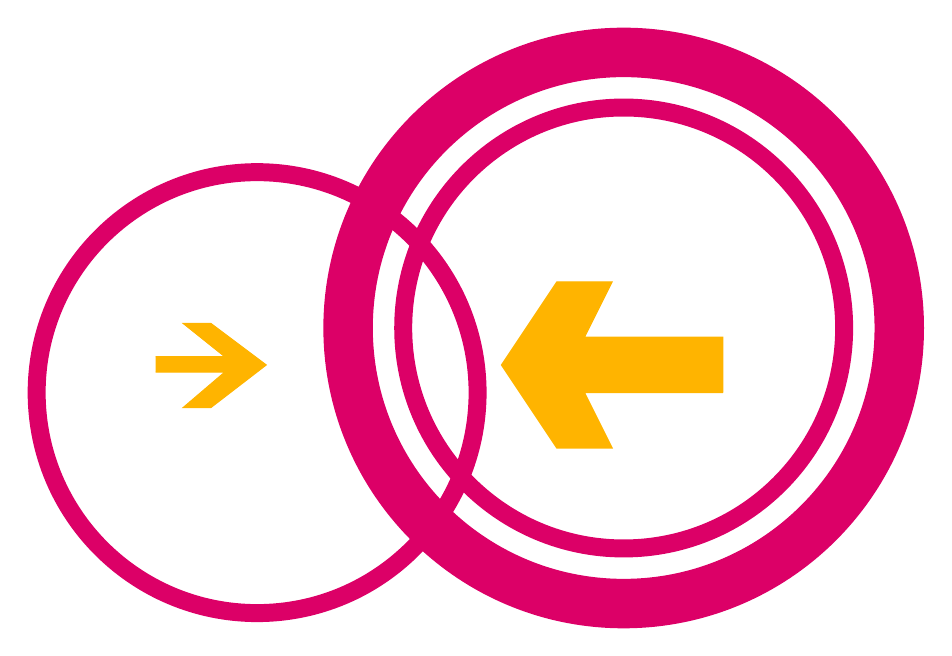
\begin{tikzpicture}[scale=2]

% ====================================================================
%
%         Kreise
%
% ====================================================================

  % Kreis schmal links
	\freifunkleft{180}

  % Kreis schmal rechts
  \freifunks{20}

  % Kreis fett rechts
	\mycircle{20}

% ====================================================================
%
%         Pfeile
%
% ====================================================================

  % Pfeil links
 
 \filldraw[fill=FFgelb, color=FFgelb]%
 %oben
(-5.25em,0.65em) -- (-4.0em,0.65em) -- (-4.75em,1.25em) -- (-4.25em,1.25em) -- %
%
(-3.25em,0.5em) % Spitze
%
% unten
-- (-4.25em,-0.27em) -- (-4.75em,-0.27em) -- (-4.0em,0.37em) %--(-6.25em,-5.0em)
-- (-5.25em,0.37em) ;

  % Pfeil rechts

  \filldraw[fill=FFgelb, color=FFgelb]
(5em,0.0em) -- (2.5em,0em) -- (3.0em,-1em) -- (2em,-1em) -- (1em,0.5em) %
-- (2em,2em) -- (3em,2em) -- (2.5em,1em) --(5em,1em)
-- (5em,0em) ;



 



\end{tikzpicture}



% Schriftzug Mitte

\huge{\FFCommunity}




\end{center}
\newpage
\Huge{\FFCommunity} \\

\small{Technische Daten: \routername} \\
\small{}
\small
\color{black}
\vspace{0.3cm}
\begin{center} 
\begin{tikzpicture}
\clip node (m) [matrix,matrix of nodes,
fill=FFmagenta!20,inner sep=0pt,
nodes in empty cells,
nodes={minimum height=1cm,minimum width=2.6cm,anchor=center,outer sep=0,font=\sffamily},
row 1/.style={nodes={fill=FFmagenta,text=white}},
column 1/.style={nodes={fill=FFmagenta,text=white,align=left,text width=3cm,text depth=0.5ex}},
column 2/.style={text width=12cm,align=left,every even row/.style={nodes={fill=white}}},
column 3/.style={text width=3cm,align=center,every even row/.style={nodes={fill=white}},},
row 1 column 1/.style={nodes={fill=FFmagenta}},%									1. spalte oben
prefix after command={[rounded corners=4mm] (m.north east) rectangle (m.south west)}
] {
& $\ \ $ tp-link-tl-wa901n-nd-v3 \
$\ \ $ CPU   			& $\ \ $ NAME \
$\ \ $ RAM 				& $\ \ $ XXX MB \
$\ \ $ Flash			& $\ \ $ XXX MB \
$\ \ $ WAN				& $\ \ $ X x1 GigE WAN	 \
$\ \ $ LAN				& $\ \ $ X x1 GigE LAN	 \
$\ \ $ USB				& $\ \ $ xX v2.0	 \
$\ \ $ WIFI 			& $\ \ $ 300 Mbit (2x2) im 2.4 Ghz Band \
						& $\ \ $ 450 Mbit (3x3) im 5 Ghz Band\
};
\end{tikzpicture}
\end{center} 


\end{document}